\documentclass[11pt,a4paper]{article}

\usepackage[margin=2.0cm]{geometry}
\usepackage{booktabs}
\usepackage{graphicx}
\usepackage{amsmath}
\usepackage{amssymb}
\usepackage{xcolor}
\usepackage{float}
\usepackage[labelfont=bf,font=small]{caption}
\usepackage[hidelinks]{hyperref}
\usepackage{enumitem}

\definecolor{bad}{HTML}{cf3a4e}
\definecolor{good}{HTML}{1f8a54}
\setlist[itemize]{leftmargin=1.4em,itemsep=2pt,topsep=3pt}
\setlist[enumerate]{leftmargin=1.6em,itemsep=5pt,topsep=3pt}
\newcommand{\num}[1]{\texttt{#1}}
\setlength{\tabcolsep}{4pt}

\newcommand{\nHolds}{5}
\newcommand{\nDatasets}{7}
\newcommand{\creditBaseTest}{0.8457}
\newcommand{\creditBaseTrain}{0.9466}
\newcommand{\creditBaseGap}{0.0974}
\newcommand{\creditKeepTest}{0.8459}
\newcommand{\creditKeepTrain}{0.8737}
\newcommand{\creditKeepGap}{0.0241}
\newcommand{\creditTree}{0.8453}
\newcommand{\creditRaw}{0.7288}
\newcommand{\creditKeepBits}{700}
\newcommand{\creditBits}{5401}
\newcommand{\creditDTest}{+0.0003}
\newcommand{\creditGapCut}{75}
\newcommand{\creditClosed}{100}
\newcommand{\creditRampTest}{0.8446}
\newcommand{\creditRampGap}{0.0431}
\newcommand{\creditCtrlTest}{0.8461}
\newcommand{\creditCtrlGap}{0.0409}
\newcommand{\creditUnifTest}{0.8460}
\newcommand{\creditUnifGap}{0.0351}
\newcommand{\creditDropFiveTest}{0.8464}
\newcommand{\creditDropFiveGap}{0.0665}
\newcommand{\creditDropFourFiveTest}{0.8460}
\newcommand{\creditDropFourFiveGap}{0.0402}
\newcommand{\creditComboTest}{0.8460}
\newcommand{\creditComboGap}{0.0271}
\newcommand{\creditBaseTrainAcc}{0.8721}
\newcommand{\creditKeepTrainAcc}{0.7930}
\newcommand{\creditBaseTestAcc}{0.7683}
\newcommand{\creditKeepTestAcc}{0.7650}
\newcommand{\creditBaseLL}{0.5086}
\newcommand{\creditKeepLL}{0.4941}
\newcommand{\creditUnifLL}{0.7787}
\newcommand{\houseSixteenHBaseTest}{0.9441}
\newcommand{\houseSixteenHBaseTrain}{0.9941}
\newcommand{\houseSixteenHBaseGap}{0.0471}
\newcommand{\houseSixteenHKeepTest}{0.9369}
\newcommand{\houseSixteenHKeepTrain}{0.9425}
\newcommand{\houseSixteenHKeepGap}{0.0034}
\newcommand{\houseSixteenHTree}{0.9526}
\newcommand{\houseSixteenHRaw}{0.8850}
\newcommand{\houseSixteenHKeepBits}{700}
\newcommand{\houseSixteenHBits}{5756}
\newcommand{\houseSixteenHDTest}{-0.0071}
\newcommand{\houseSixteenHGapCut}{93}
\newcommand{\houseSixteenHClosed}{87}
\newcommand{\houseSixteenHRampTest}{0.9437}
\newcommand{\houseSixteenHRampGap}{0.0206}
\newcommand{\houseSixteenHCtrlTest}{0.9440}
\newcommand{\houseSixteenHCtrlGap}{0.0192}
\newcommand{\houseSixteenHUnifTest}{0.9437}
\newcommand{\houseSixteenHUnifGap}{0.0149}
\newcommand{\houseSixteenHDropFiveTest}{0.9439}
\newcommand{\houseSixteenHDropFiveGap}{0.0345}
\newcommand{\houseSixteenHDropFourFiveTest}{0.9415}
\newcommand{\houseSixteenHDropFourFiveGap}{0.0184}
\newcommand{\houseSixteenHComboTest}{0.9400}
\newcommand{\houseSixteenHComboGap}{0.0086}
\newcommand{\houseSixteenHBaseTrainAcc}{0.9619}
\newcommand{\houseSixteenHKeepTrainAcc}{0.8733}
\newcommand{\houseSixteenHBaseTestAcc}{0.8765}
\newcommand{\houseSixteenHKeepTestAcc}{0.8651}
\newcommand{\houseSixteenHBaseLL}{0.3170}
\newcommand{\houseSixteenHKeepLL}{0.3205}
\newcommand{\houseSixteenHUnifLL}{0.4234}
\newcommand{\MagicTelescopeBaseTest}{0.9047}
\newcommand{\MagicTelescopeBaseTrain}{0.9678}
\newcommand{\MagicTelescopeBaseGap}{0.0627}
\newcommand{\MagicTelescopeKeepTest}{0.8994}
\newcommand{\MagicTelescopeKeepTrain}{0.9041}
\newcommand{\MagicTelescopeKeepGap}{0.0037}
\newcommand{\MagicTelescopeTree}{0.9377}
\newcommand{\MagicTelescopeRaw}{0.8486}
\newcommand{\MagicTelescopeKeepBits}{698}
\newcommand{\MagicTelescopeBits}{4684}
\newcommand{\MagicTelescopeDTest}{-0.0053}
\newcommand{\MagicTelescopeGapCut}{94}
\newcommand{\MagicTelescopeClosed}{63}
\newcommand{\MagicTelescopeRampTest}{0.9032}
\newcommand{\MagicTelescopeRampGap}{0.0198}
\newcommand{\MagicTelescopeCtrlTest}{0.9040}
\newcommand{\MagicTelescopeCtrlGap}{0.0196}
\newcommand{\MagicTelescopeUnifTest}{0.9029}
\newcommand{\MagicTelescopeUnifGap}{0.0151}
\newcommand{\MagicTelescopeDropFiveTest}{0.9050}
\newcommand{\MagicTelescopeDropFiveGap}{0.0417}
\newcommand{\MagicTelescopeDropFourFiveTest}{0.9030}
\newcommand{\MagicTelescopeDropFourFiveGap}{0.0224}
\newcommand{\MagicTelescopeComboTest}{0.9004}
\newcommand{\MagicTelescopeComboGap}{0.0096}
\newcommand{\MagicTelescopeBaseTrainAcc}{0.9096}
\newcommand{\MagicTelescopeKeepTrainAcc}{0.8227}
\newcommand{\MagicTelescopeBaseTestAcc}{0.8251}
\newcommand{\MagicTelescopeKeepTestAcc}{0.8281}
\newcommand{\MagicTelescopeBaseLL}{0.3935}
\newcommand{\MagicTelescopeKeepLL}{0.4010}
\newcommand{\MagicTelescopeUnifLL}{0.5237}
\newcommand{\pendigitsBaseTest}{0.9986}
\newcommand{\pendigitsBaseTrain}{1.0000}
\newcommand{\pendigitsBaseGap}{0.0015}
\newcommand{\pendigitsKeepTest}{0.9971}
\newcommand{\pendigitsKeepTrain}{0.9993}
\newcommand{\pendigitsKeepGap}{0.0023}
\newcommand{\pendigitsTree}{0.9995}
\newcommand{\pendigitsRaw}{0.9906}
\newcommand{\pendigitsKeepBits}{700}
\newcommand{\pendigitsBits}{5517}
\newcommand{\pendigitsDTest}{-0.0015}
\newcommand{\pendigitsGapCut}{n/a}
\newcommand{\pendigitsClosed}{91}
\newcommand{\pendigitsRampTest}{0.9979}
\newcommand{\pendigitsRampGap}{0.0021}
\newcommand{\pendigitsCtrlTest}{0.9978}
\newcommand{\pendigitsCtrlGap}{0.0021}
\newcommand{\pendigitsUnifTest}{0.9974}
\newcommand{\pendigitsUnifGap}{0.0023}
\newcommand{\pendigitsDropFiveTest}{0.9985}
\newcommand{\pendigitsDropFiveGap}{0.0016}
\newcommand{\pendigitsDropFourFiveTest}{0.9983}
\newcommand{\pendigitsDropFourFiveGap}{0.0020}
\newcommand{\pendigitsComboTest}{0.9977}
\newcommand{\pendigitsComboGap}{0.0023}
\newcommand{\pendigitsBaseTrainAcc}{1.0000}
\newcommand{\pendigitsKeepTrainAcc}{0.9696}
\newcommand{\pendigitsBaseTestAcc}{0.9703}
\newcommand{\pendigitsKeepTestAcc}{0.9303}
\newcommand{\pendigitsBaseLL}{0.1093}
\newcommand{\pendigitsKeepLL}{0.2202}
\newcommand{\pendigitsUnifLL}{0.2168}
\newcommand{\covertypeBaseTest}{0.9370}
\newcommand{\covertypeBaseTrain}{0.9890}
\newcommand{\covertypeBaseGap}{0.0497}
\newcommand{\covertypeKeepTest}{0.9290}
\newcommand{\covertypeKeepTrain}{0.9505}
\newcommand{\covertypeKeepGap}{0.0191}
\newcommand{\covertypeTree}{0.9654}
\newcommand{\covertypeRaw}{0.9106}
\newcommand{\covertypeKeepBits}{689}
\newcommand{\covertypeBits}{4339}
\newcommand{\covertypeDTest}{-0.0081}
\newcommand{\covertypeGapCut}{62}
\newcommand{\covertypeClosed}{48}
\newcommand{\covertypeRampTest}{0.9345}
\newcommand{\covertypeRampGap}{0.0306}
\newcommand{\covertypeCtrlTest}{0.9339}
\newcommand{\covertypeCtrlGap}{0.0298}
\newcommand{\covertypeUnifTest}{0.9332}
\newcommand{\covertypeUnifGap}{0.0267}
\newcommand{\covertypeDropFiveTest}{0.9368}
\newcommand{\covertypeDropFiveGap}{0.0398}
\newcommand{\covertypeDropFourFiveTest}{0.9354}
\newcommand{\covertypeDropFourFiveGap}{0.0303}
\newcommand{\covertypeComboTest}{0.9329}
\newcommand{\covertypeComboGap}{0.0223}
\newcommand{\covertypeBaseTrainAcc}{0.8956}
\newcommand{\covertypeKeepTrainAcc}{0.7438}
\newcommand{\covertypeBaseTestAcc}{0.7233}
\newcommand{\covertypeKeepTestAcc}{0.7179}
\newcommand{\covertypeBaseLL}{0.6434}
\newcommand{\covertypeKeepLL}{0.6644}
\newcommand{\covertypeUnifLL}{0.7488}
\newcommand{\cpuactBaseTest}{0.9758}
\newcommand{\cpuactBaseTrain}{0.9912}
\newcommand{\cpuactBaseGap}{0.0092}
\newcommand{\cpuactKeepTest}{0.9599}
\newcommand{\cpuactKeepTrain}{0.9634}
\newcommand{\cpuactKeepGap}{-0.0015}
\newcommand{\cpuactTree}{0.9867}
\newcommand{\cpuactRaw}{0.7638}
\newcommand{\cpuactKeepBits}{629}
\newcommand{\cpuactBits}{3507}
\newcommand{\cpuactDTest}{-0.0159}
\newcommand{\cpuactGapCut}{116}
\newcommand{\cpuactClosed}{95}
\newcommand{\cpuactRampTest}{0.8253}
\newcommand{\cpuactRampGap}{-0.0171}
\newcommand{\cpuactCtrlTest}{-0.7046}
\newcommand{\cpuactCtrlGap}{-0.2453}
\newcommand{\cpuactUnifTest}{-1.9647}
\newcommand{\cpuactUnifGap}{-0.4247}
\newcommand{\cpuactDropFiveTest}{0.9737}
\newcommand{\cpuactDropFiveGap}{0.0043}
\newcommand{\cpuactDropFourFiveTest}{0.9677}
\newcommand{\cpuactDropFourFiveGap}{0.0015}
\newcommand{\cpuactComboTest}{0.9393}
\newcommand{\cpuactComboGap}{-0.0040}
\newcommand{\winequalityBaseTest}{0.2854}
\newcommand{\winequalityBaseTrain}{0.9199}
\newcommand{\winequalityBaseGap}{0.6045}
\newcommand{\winequalityKeepTest}{0.2793}
\newcommand{\winequalityKeepTrain}{0.4096}
\newcommand{\winequalityKeepGap}{0.1180}
\newcommand{\winequalityTree}{0.4722}
\newcommand{\winequalityRaw}{0.2800}
\newcommand{\winequalityKeepBits}{700}
\newcommand{\winequalityBits}{5498}
\newcommand{\winequalityDTest}{-0.0061}
\newcommand{\winequalityGapCut}{80}
\newcommand{\winequalityClosed}{3}
\newcommand{\winequalityRampTest}{0.2577}
\newcommand{\winequalityRampGap}{0.1805}
\newcommand{\winequalityCtrlTest}{0.2267}
\newcommand{\winequalityCtrlGap}{0.1732}
\newcommand{\winequalityUnifTest}{0.1518}
\newcommand{\winequalityUnifGap}{0.1190}
\newcommand{\winequalityDropFiveTest}{0.3075}
\newcommand{\winequalityDropFiveGap}{0.4303}
\newcommand{\winequalityDropFourFiveTest}{0.3071}
\newcommand{\winequalityDropFourFiveGap}{0.2274}
\newcommand{\winequalityComboTest}{0.2890}
\newcommand{\winequalityComboGap}{0.1254}
% ---- overview table (generated) ----
\newcommand{\taboverview}{%
\begin{tabular}{llrrrrrrrrrc}
\toprule
\textbf{Dataset} & \textbf{Kind} & \textbf{Best tree} & \textbf{Raw only} & \multicolumn{3}{c}{\textbf{All bits}} & \multicolumn{3}{c}{\textbf{Keep depths 0--2}} & \textbf{Test change} & \textbf{Holds}\\
\cmidrule(lr){5-7}\cmidrule(lr){8-10}
 & & & & train & test & gap & train & test & gap & & \\
\midrule
credit & two-class & 0.8453 & 0.7288 & 0.9466 & 0.8457 & 0.0974 & 0.8737 & 0.8459 & 0.0241 & +0.0003 & yes\\
house\_16H & two-class & 0.9526 & 0.8850 & 0.9941 & 0.9441 & 0.0471 & 0.9425 & 0.9369 & 0.0034 & -0.0071 & yes\\
MagicTelescope & two-class & 0.9377 & 0.8486 & 0.9678 & 0.9047 & 0.0627 & 0.9041 & 0.8994 & 0.0037 & -0.0053 & yes\\
pendigits & ten-class & 0.9995 & 0.9906 & 1.0000 & 0.9986 & 0.0015 & 0.9993 & 0.9971 & 0.0023 & -0.0015 & no\\
covertype & seven-class & 0.9654 & 0.9106 & 0.9890 & 0.9370 & 0.0497 & 0.9505 & 0.9290 & 0.0191 & -0.0081 & yes\\
cpu\_act & regression & 0.9867 & 0.7638 & 0.9912 & 0.9758 & 0.0092 & 0.9634 & 0.9599 & -0.0015 & -0.0159 & no\\
wine\_quality & regression & 0.4722 & 0.2800 & 0.9199 & 0.2854 & 0.6045 & 0.4096 & 0.2793 & 0.1180 & -0.0061 & yes\\
\bottomrule
\end{tabular}}

% ---- credit (generated) ----
\newcommand{\tabcredit}{%
\begin{tabular}{lrrrrrrrrr}
\toprule
\textbf{Arm} & \textbf{Bits} & \textbf{Flip} & \multicolumn{3}{c}{\textbf{Ranking score}} & \textbf{Gap} & \multicolumn{2}{c}{\textbf{Accuracy}} & \textbf{Log loss}\\
\cmidrule(lr){4-6}\cmidrule(lr){8-9}
 & & rate & train & val & test & & train & test & test\\
\midrule
raw features only (no tree bits) & 10 & -- & 0.7466 & 0.7317 & 0.7288 & +0.0149 & 0.6674 & 0.6496 & 0.6310\\
\midrule
all bits, no change & 5401 & -- & 0.9466 & 0.8492 & 0.8457 & +0.0974 & 0.8721 & 0.7683 & 0.5086\\
flip every bit, p = 0.20 & 5401 & 0.200 & 0.8840 & 0.8489 & 0.8460 & +0.0351 & 0.7562 & 0.7338 & 0.7787\\
flips rising with depth, P = 0.2 & 5401 & 0.159 & 0.8914 & 0.8483 & 0.8446 & +0.0431 & 0.7911 & 0.7588 & 0.5861\\
flip every bit, p = 0.16 (same budget as the ramp) & 5401 & 0.160 & 0.8899 & 0.8490 & 0.8461 & +0.0409 & 0.7722 & 0.7429 & 0.6733\\
delete depth 5 & 2935 & -- & 0.9162 & 0.8497 & 0.8464 & +0.0665 & 0.8355 & 0.7675 & 0.4993\\
delete depths 4 and 5 & 1480 & -- & 0.8899 & 0.8497 & 0.8460 & +0.0402 & 0.8096 & 0.7675 & 0.4955\\
delete 4 and 5, then ramp 0.2 & 1480 & 0.025 & 0.8763 & 0.8491 & 0.8460 & +0.0271 & 0.7857 & 0.7650 & 0.5142\\
\textbf{keep only depths 0, 1, 2} & 700 & -- & 0.8737 & 0.8496 & 0.8459 & +0.0241 & 0.7930 & 0.7650 & 0.4941\\
\midrule
best tree model (lightgbm) & & & & & 0.8453 & & & & \\
\bottomrule
\end{tabular}}

% ---- house_16H (generated) ----
\newcommand{\tabhouseSixteenH}{%
\begin{tabular}{lrrrrrrrrr}
\toprule
\textbf{Arm} & \textbf{Bits} & \textbf{Flip} & \multicolumn{3}{c}{\textbf{Ranking score}} & \textbf{Gap} & \multicolumn{2}{c}{\textbf{Accuracy}} & \textbf{Log loss}\\
\cmidrule(lr){4-6}\cmidrule(lr){8-9}
 & & rate & train & val & test & & train & test & test\\
\midrule
raw features only (no tree bits) & 16 & -- & 0.8856 & 0.8869 & 0.8850 & -0.0012 & 0.8156 & 0.8182 & 0.4578\\
\midrule
all bits, no change & 5756 & -- & 0.9941 & 0.9471 & 0.9441 & +0.0471 & 0.9619 & 0.8765 & 0.3170\\
flip every bit, p = 0.20 & 5756 & 0.200 & 0.9611 & 0.9462 & 0.9437 & +0.0149 & 0.8811 & 0.8651 & 0.4234\\
flips rising with depth, P = 0.2 & 5756 & 0.161 & 0.9671 & 0.9465 & 0.9437 & +0.0206 & 0.8941 & 0.8671 & 0.3623\\
flip every bit, p = 0.16 (same budget as the ramp) & 5756 & 0.160 & 0.9659 & 0.9467 & 0.9440 & +0.0192 & 0.8925 & 0.8681 & 0.3835\\
delete depth 5 & 3032 & -- & 0.9808 & 0.9463 & 0.9439 & +0.0345 & 0.9323 & 0.8755 & 0.3082\\
delete depths 4 and 5 & 1497 & -- & 0.9625 & 0.9440 & 0.9415 & +0.0184 & 0.8995 & 0.8701 & 0.3090\\
delete 4 and 5, then ramp 0.2 & 1497 & 0.024 & 0.9517 & 0.9431 & 0.9400 & +0.0086 & 0.8816 & 0.8715 & 0.3203\\
\textbf{keep only depths 0, 1, 2} & 700 & -- & 0.9425 & 0.9392 & 0.9369 & +0.0034 & 0.8733 & 0.8651 & 0.3205\\
\midrule
best tree model (lightgbm) & & & & & 0.9526 & & & & \\
\bottomrule
\end{tabular}}

% ---- MagicTelescope (generated) ----
\newcommand{\tabMagicTelescope}{%
\begin{tabular}{lrrrrrrrrr}
\toprule
\textbf{Arm} & \textbf{Bits} & \textbf{Flip} & \multicolumn{3}{c}{\textbf{Ranking score}} & \textbf{Gap} & \multicolumn{2}{c}{\textbf{Accuracy}} & \textbf{Log loss}\\
\cmidrule(lr){4-6}\cmidrule(lr){8-9}
 & & rate & train & val & test & & train & test & test\\
\midrule
raw features only (no tree bits) & 10 & -- & 0.8418 & 0.8376 & 0.8486 & +0.0042 & 0.7724 & 0.7698 & 0.4835\\
\midrule
all bits, no change & 4684 & -- & 0.9678 & 0.9051 & 0.9047 & +0.0627 & 0.9096 & 0.8251 & 0.3935\\
flip every bit, p = 0.20 & 4684 & 0.200 & 0.9184 & 0.9033 & 0.9029 & +0.0151 & 0.8343 & 0.8186 & 0.5237\\
flips rising with depth, P = 0.2 & 4684 & 0.155 & 0.9247 & 0.9049 & 0.9032 & +0.0198 & 0.8470 & 0.8216 & 0.4411\\
flip every bit, p = 0.16 (same budget as the ramp) & 4684 & 0.160 & 0.9240 & 0.9045 & 0.9040 & +0.0196 & 0.8455 & 0.8246 & 0.4747\\
delete depth 5 & 2752 & -- & 0.9470 & 0.9054 & 0.9050 & +0.0417 & 0.8787 & 0.8296 & 0.3892\\
delete depths 4 and 5 & 1454 & -- & 0.9257 & 0.9033 & 0.9030 & +0.0224 & 0.8514 & 0.8271 & 0.3925\\
delete 4 and 5, then ramp 0.2 & 1454 & 0.028 & 0.9110 & 0.9014 & 0.9004 & +0.0096 & 0.8323 & 0.8236 & 0.4042\\
\textbf{keep only depths 0, 1, 2} & 698 & -- & 0.9041 & 0.9005 & 0.8994 & +0.0037 & 0.8227 & 0.8281 & 0.4010\\
\midrule
best tree model (xgboost) & & & & & 0.9377 & & & & \\
\bottomrule
\end{tabular}}

% ---- pendigits (generated) ----
\newcommand{\tabpendigits}{%
\begin{tabular}{lrrrrrrrrr}
\toprule
\textbf{Arm} & \textbf{Bits} & \textbf{Flip} & \multicolumn{3}{c}{\textbf{Ranking score}} & \textbf{Gap} & \multicolumn{2}{c}{\textbf{Accuracy}} & \textbf{Log loss}\\
\cmidrule(lr){4-6}\cmidrule(lr){8-9}
 & & rate & train & val & test & & train & test & test\\
\midrule
raw features only (no tree bits) & 16 & -- & 0.9911 & 0.9911 & 0.9906 & -0.0001 & 0.8980 & 0.9005 & 0.4524\\
\midrule
all bits, no change & 5517 & -- & 1.0000 & 0.9985 & 0.9986 & +0.0015 & 1.0000 & 0.9703 & 0.1093\\
flip every bit, p = 0.20 & 5517 & 0.200 & 0.9996 & 0.9973 & 0.9974 & +0.0023 & 0.9645 & 0.9375 & 0.2168\\
flips rising with depth, P = 0.2 & 5517 & 0.159 & 0.9999 & 0.9978 & 0.9979 & +0.0021 & 0.9818 & 0.9478 & 0.1628\\
flip every bit, p = 0.16 (same budget as the ramp) & 5517 & 0.160 & 0.9999 & 0.9977 & 0.9978 & +0.0021 & 0.9783 & 0.9460 & 0.1745\\
delete depth 5 & 3024 & -- & 1.0000 & 0.9984 & 0.9985 & +0.0016 & 1.0000 & 0.9648 & 0.1211\\
delete depths 4 and 5 & 1498 & -- & 1.0000 & 0.9980 & 0.9983 & +0.0020 & 0.9960 & 0.9557 & 0.1493\\
delete 4 and 5, then ramp 0.2 & 1498 & 0.025 & 0.9997 & 0.9974 & 0.9977 & +0.0023 & 0.9727 & 0.9466 & 0.1715\\
\textbf{keep only depths 0, 1, 2} & 700 & -- & 0.9993 & 0.9969 & 0.9971 & +0.0023 & 0.9696 & 0.9303 & 0.2202\\
\midrule
best tree model (lightgbm) & & & & & 0.9995 & & & & \\
\bottomrule
\end{tabular}}

% ---- covertype (generated) ----
\newcommand{\tabcovertype}{%
\begin{tabular}{lrrrrrrrrr}
\toprule
\textbf{Arm} & \textbf{Bits} & \textbf{Flip} & \multicolumn{3}{c}{\textbf{Ranking score}} & \textbf{Gap} & \multicolumn{2}{c}{\textbf{Accuracy}} & \textbf{Log loss}\\
\cmidrule(lr){4-6}\cmidrule(lr){8-9}
 & & rate & train & val & test & & train & test & test\\
\midrule
raw features only (no tree bits) & 54 & -- & 0.9238 & 0.9188 & 0.9106 & +0.0050 & 0.6970 & 0.6979 & 0.7367\\
\midrule
all bits, no change & 4339 & -- & 0.9890 & 0.9394 & 0.9370 & +0.0497 & 0.8956 & 0.7233 & 0.6434\\
flip every bit, p = 0.20 & 4339 & 0.200 & 0.9619 & 0.9352 & 0.9332 & +0.0267 & 0.7696 & 0.7163 & 0.7488\\
flips rising with depth, P = 0.2 & 4339 & 0.154 & 0.9675 & 0.9369 & 0.9345 & +0.0306 & 0.7871 & 0.7196 & 0.6931\\
flip every bit, p = 0.16 (same budget as the ramp) & 4339 & 0.160 & 0.9662 & 0.9364 & 0.9339 & +0.0298 & 0.7804 & 0.7179 & 0.7116\\
delete depth 5 & 2554 & -- & 0.9797 & 0.9399 & 0.9368 & +0.0398 & 0.8435 & 0.7233 & 0.6331\\
delete depths 4 and 5 & 1394 & -- & 0.9670 & 0.9367 & 0.9354 & +0.0303 & 0.7925 & 0.7238 & 0.6350\\
delete 4 and 5, then ramp 0.2 & 1394 & 0.029 & 0.9561 & 0.9337 & 0.9329 & +0.0223 & 0.7578 & 0.7179 & 0.6512\\
\textbf{keep only depths 0, 1, 2} & 689 & -- & 0.9505 & 0.9314 & 0.9290 & +0.0191 & 0.7438 & 0.7179 & 0.6644\\
\midrule
best tree model (xgboost) & & & & & 0.9654 & & & & \\
\bottomrule
\end{tabular}}

% ---- cpu_act (generated) ----
\newcommand{\tabcpuact}{%
\begin{tabular}{lrrrrrrrrr}
\toprule
\textbf{Arm} & \textbf{Bits} & \textbf{Flip} & \multicolumn{3}{c}{\textbf{Explained variance}} & \textbf{Gap} & \multicolumn{2}{c}{\textbf{Typical error}} & \textbf{Avg.\ abs.\ error}\\
\cmidrule(lr){4-6}\cmidrule(lr){8-9}
 & & rate & train & val & test & & train & test & test\\
\midrule
raw features only (no tree bits) & 21 & -- & 0.7247 & 0.7070 & 0.7638 & +0.0177 & 9.540 & 8.974 & 5.695\\
\midrule
all bits, no change & 3507 & -- & 0.9912 & 0.9820 & 0.9758 & +0.0092 & 1.707 & 2.874 & 1.956\\
flip every bit, p = 0.20 & 3507 & 0.200 & -2.0525 & -1.6278 & -1.9647 & -0.4247 & 31.765 & 31.794 & 30.880\\
flips rising with depth, P = 0.2 & 3507 & 0.153 & 0.8285 & 0.8456 & 0.8253 & -0.0171 & 7.529 & 7.718 & 6.828\\
flip every bit, p = 0.16 (same budget as the ramp) & 3507 & 0.160 & -0.7566 & -0.5114 & -0.7046 & -0.2453 & 24.097 & 24.109 & 23.398\\
delete depth 5 & 1939 & -- & 0.9849 & 0.9805 & 0.9737 & +0.0043 & 2.236 & 2.997 & 2.039\\
delete depths 4 and 5 & 1116 & -- & 0.9770 & 0.9755 & 0.9677 & +0.0015 & 2.757 & 3.318 & 2.296\\
delete 4 and 5, then ramp 0.2 & 1116 & 0.026 & 0.9433 & 0.9472 & 0.9393 & -0.0040 & 4.331 & 4.549 & 3.461\\
\textbf{keep only depths 0, 1, 2} & 629 & -- & 0.9634 & 0.9648 & 0.9599 & -0.0015 & 3.480 & 3.700 & 2.632\\
\midrule
best tree model (lightgbm) & & & & & 0.9867 & & & & \\
\bottomrule
\end{tabular}}

% ---- wine_quality (generated) ----
\newcommand{\tabwinequality}{%
\begin{tabular}{lrrrrrrrrr}
\toprule
\textbf{Arm} & \textbf{Bits} & \textbf{Flip} & \multicolumn{3}{c}{\textbf{Explained variance}} & \textbf{Gap} & \multicolumn{2}{c}{\textbf{Typical error}} & \textbf{Avg.\ abs.\ error}\\
\cmidrule(lr){4-6}\cmidrule(lr){8-9}
 & & rate & train & val & test & & train & test & test\\
\midrule
raw features only (no tree bits) & 11 & -- & 0.2936 & 0.2945 & 0.2800 & -0.0008 & 0.731 & 0.748 & 0.586\\
\midrule
all bits, no change & 5498 & -- & 0.9199 & 0.3153 & 0.2854 & +0.6045 & 0.246 & 0.745 & 0.585\\
flip every bit, p = 0.20 & 5498 & 0.200 & 0.3219 & 0.2030 & 0.1518 & +0.1190 & 0.716 & 0.812 & 0.640\\
flips rising with depth, P = 0.2 & 5498 & 0.159 & 0.4797 & 0.2992 & 0.2577 & +0.1805 & 0.628 & 0.760 & 0.595\\
flip every bit, p = 0.16 (same budget as the ramp) & 5498 & 0.160 & 0.4374 & 0.2642 & 0.2267 & +0.1732 & 0.653 & 0.775 & 0.607\\
delete depth 5 & 2993 & -- & 0.7358 & 0.3055 & 0.3075 & +0.4303 & 0.447 & 0.734 & 0.575\\
delete depths 4 and 5 & 1493 & -- & 0.5443 & 0.3169 & 0.3071 & +0.2274 & 0.587 & 0.734 & 0.570\\
delete 4 and 5, then ramp 0.2 & 1493 & 0.025 & 0.4370 & 0.3116 & 0.2890 & +0.1254 & 0.653 & 0.744 & 0.577\\
\textbf{keep only depths 0, 1, 2} & 700 & -- & 0.4096 & 0.2916 & 0.2793 & +0.1180 & 0.668 & 0.749 & 0.585\\
\midrule
best tree model (random forest) & & & & & 0.4722 & & & & \\
\bottomrule
\end{tabular}}

% ---- sizes (generated) ----
\newcommand{\tabsizes}{%
\begin{tabular}{llrrrrrr}
\toprule
\textbf{Dataset} & \textbf{Kind} & \textbf{Raw features} & \textbf{Train} & \textbf{Val} & \textbf{Test} & \textbf{Tree bits} & \textbf{Best tree}\\
\midrule
credit & two-class & 10 & 11,200 & 2,400 & 2,400 & 5,401 & lightgbm 0.8453\\
house\_16H & two-class & 16 & 9,441 & 2,023 & 2,024 & 5,756 & lightgbm 0.9526\\
MagicTelescope & two-class & 10 & 9,363 & 2,006 & 2,007 & 4,684 & xgboost 0.9377\\
pendigits & ten-class & 16 & 7,694 & 1,649 & 1,649 & 5,517 & lightgbm 0.9995\\
covertype & seven-class & 54 & 11,200 & 2,400 & 2,400 & 4,339 & xgboost 0.9654\\
cpu\_act & regression & 21 & 5,734 & 1,229 & 1,229 & 3,507 & lightgbm 0.9867\\
wine\_quality & regression & 11 & 4,547 & 975 & 975 & 5,498 & random forest 0.4722\\
\bottomrule
\end{tabular}}

\title{\vspace{-1.6cm}\textbf{Does Feature Regularisation Hold Beyond One Dataset?}\\
\large Seven datasets, three kinds of problem, every factor held fixed}
\author{Experiment report}
\date{\small 27 September 2026}

\begin{document}
\maketitle
\vspace{-0.8cm}

\begin{center}
\fbox{\begin{minipage}{0.95\textwidth}
\small\textbf{Summary.} The earlier credit experiment showed two things: a simple
linear model on the tree bits matched the best tree model, and removing the
deepest tree layers cut overfitting more than tenfold at no cost. This report
repeats the same experiment, with every setting held identical, on seven
datasets covering two-class, many-class and number-prediction problems.
\textbf{The regularisation result holds}: on every dataset where the model
overfit, deleting the deep layers cut the train-minus-validation gap by 62 to
94 percent, and the training score came down toward the test score, for a
test cost never above \num{0.016}. \textbf{The ``matches the tree'' result
does not generalise}: credit is the only dataset where the linear model reaches
the best tree; elsewhere it covers between 48 and 95 percent of the way from
raw features to the tree, and on wine quality almost none. \textbf{Deleting
beats flipping}: bit-flip noise damages calibration on classification and is
destructive on regression, while deletion regularises without side effects.
\end{minipage}}
\end{center}

\section{Goal of the experiment}

The previous report studied one dataset, credit. With the classifier fixed to
a plain logistic regression on the bits of a frozen random forest, two results
stood out. First, the linear model matched the best gradient-boosted tree
(\num{0.8457} against \num{0.8453} on the ranking score). Second, regularising
the \emph{features} rather than the model, by deleting the deepest tree layers
or flipping bits during training, reduced the train-minus-validation gap from
\num{0.0974} to as little as \num{0.0092} with no change in the test score.

The response to that report set five requirements, and this experiment is
built to meet each of them.

\begin{enumerate}
  \item \textbf{Try it on a few more datasets.} Six new datasets were added to
        credit, chosen to cover two-class problems, many-class problems and
        number-prediction (regression) problems.
  \item \textbf{Keep all experimental factors intact.} The forest, the honesty
        protocol, the head and its penalty, the noise recipe, the row cap, the
        random seed and the set of arms are identical on every dataset. Nothing
        was tuned per dataset.
  \item \textbf{Track all metrics across train, validation and test.} Every run
        reports three scores on all three splits.
  \item \textbf{Report that the training accuracy fell from 1.} The tables show
        training and test side by side for the full encoding and for the
        shallow one, so the drop is visible directly.
  \item \textbf{See whether the observation holds.} Each dataset gets an
        explicit yes-or-no verdict against a rule fixed before the runs.
\end{enumerate}

The question, in one line: \emph{is ``regularise the features, not the model''
a property of credit, or a property of tree encodings in general?}

\section{Datasets}

Seven datasets, all from public benchmark collections and all without the
identifier-column leakage that spoiled an earlier dataset in this project. Each
was split into 70 percent training, 15 percent validation and 15 percent test,
with the same random seed, and capped at \num{16000} rows.

\begin{table}[H]\centering\small
\begin{tabular}{lp{11.2cm}}
\toprule
\textbf{Dataset} & \textbf{What the model has to predict}\\
\midrule
credit & Whether a person will fall seriously behind on loan payments within two years, from ten numbers describing their finances. Two classes, balanced. The anchor dataset from the previous report.\\
house\_16H & Whether a house is worth more than the typical house in its area, from sixteen census-style numbers. Two classes.\\
MagicTelescope & Whether a flash recorded by a gamma-ray telescope is a real signal or background noise, from ten shape measurements of the flash. Two classes.\\
pendigits & Which digit from 0 to 9 was written, from sixteen numbers describing the pen's path. Ten classes, balanced.\\
covertype & Which of seven forest cover types grows on a patch of land, from fifty-four map-derived measurements. Seven classes, unbalanced. The full dataset has 581,012 rows; a random 16,000 were used.\\
cpu\_act & The fraction of time a computer's processor spends running user programs, from twenty-one activity counters. A number to predict.\\
wine\_quality & The quality score (3 to 9) that a taster gave a wine, from eleven chemical measurements. A number to predict, and known to be difficult.\\
\bottomrule
\end{tabular}
\end{table}

\begin{table}[H]\centering\small
\tabsizes
\caption{Sizes after the split, the width of the tree encoding each forest
produced, and the best of the three reference tree models fitted on the raw
features of the same split. ``Kind'' names the type of problem.}
\end{table}

\paragraph{How the scores are read.} Three kinds of problem need slightly
different scores, and all are reported on all three splits.

\begin{itemize}
  \item \textbf{Ranking score} (classification). How well the model puts the
        positive cases above the negative ones when sorted by its predicted
        probability. A value of \num{0.5} is a coin flip and \num{1.0} is
        perfect. For many-class problems it is computed one class against the
        rest and averaged. This is the primary score for classification.
  \item \textbf{Accuracy} (classification). The fraction of rows the model
        labels correctly. \textbf{Log loss} (classification). A penalty for
        being confidently wrong; lower is better. It measures how well
        calibrated the predicted probabilities are, which the ranking score
        ignores.
  \item \textbf{Explained-variance score} (regression). How much of the spread
        in the target the predictions account for. \num{1.0} is perfect,
        \num{0} means no better than always guessing the average, and a negative
        value means worse than that. This is the primary score for regression.
        Alongside it, the \textbf{typical error} (the root of the mean squared
        error) and the \textbf{average absolute error}, both in the target's
        own units.
\end{itemize}

\paragraph{Reference tree models.} Three tree models were fitted on the raw
features of each split with default settings: gradient-boosted trees from two
popular libraries (XGBoost and LightGBM) and a random forest. The best of the
three on the test split is called ``the best tree'' throughout and marks the
target every other number is compared to.

\section{Training architecture and methodology}

Every model in this report has two stages. The first is fitted once and then
frozen. The second is the only thing that learns.

\paragraph{Stage 1: the tree encoding.} A random forest of \num{100} trees is
fitted on the training split, with each tree allowed to grow six levels deep
and each leaf required to hold at least five rows. For regression problems the
forest is a regression forest; otherwise a classification forest. Every
decision node inside every tree becomes one yes-or-no feature, which we call a
\emph{bit}: it is 1 if the row goes left at that node and 0 otherwise. Across
the whole forest this gives between \num{3507} and \num{5756} bits per row,
depending on the dataset. The forest is never touched again; it is a way of
describing rows, not a predictor.

\paragraph{Depth means reliability.} A node near the top of a tree was chosen
by looking at thousands of rows. A node at the bottom was chosen by looking at
a few dozen. On credit, splits at depths 0 to 2 were fitted on a median of
2,355 rows each, while the deeper splits were fitted on a median of 208. The
deep bits are therefore the memorised part of the forest, and roughly half of
all bits sit in the single deepest layer. This is why the interventions below
are organised by depth.

\paragraph{Honest bits.} The forest was fitted using the training labels, so a
training row's bits from trees whose random sample \emph{contained} that row
were partly carved to classify that very row. Test rows have no such trees. To
remove this asymmetry, each training row keeps only the bits from trees that
never saw it, on average \num{36.8} of the 100, rescaled so that magnitudes
match. Validation and test rows use all trees. This protocol is identical on
every dataset and arm.

\paragraph{Stage 2: the head.} A convex linear model with one weight per bit,
no hidden layer and no nonlinearity, solved exactly. For classification it is a
logistic regression, extended in the usual way to many classes. For regression
it is a ridge regression, with the penalty set so the weight on the penalty
term matches the classification setting. There is no learning rate, no number
of training rounds and no random initialisation anywhere, so no result can be
blamed on the optimiser.

\paragraph{The penalty is fixed.} The penalty setting is $C = 0.01$ everywhere.
A small $C$ means a strong pull of the weights toward zero. It was deliberately
not tuned per dataset or per arm, because that would leave any difference in
the tables attributable either to the features or to a differently tuned
penalty. Holding it fixed makes every difference attributable to the features
alone.

\paragraph{How noise is applied.} A convex solver sees one fixed table of
numbers, so it cannot draw fresh random flips at every training step the way a
neural network trainer can. The equivalent is to build three independently
flipped copies of the training rows and fit on all of them together, which
approximates minimising the loss averaged over the noise. Because stacking
three copies triples the data term of the objective, the penalty is rescaled
by three so that the pull per original training row is the same as in the
arms without noise. Flips are applied to the plain 0/1 bits before the honesty
mask. \textbf{Validation and test always see clean, unflipped bits.}

\paragraph{How deletion is applied.} Deleting a depth means dropping every bit
at that depth as a column, from training, validation and test alike. A deleted
bit can never be flipped back in. Deletion is a permanent change to the input,
so it needs no noisy copies and no rescaling.

\paragraph{How overfitting is measured.} The gap is the training score minus
the validation score on the primary metric, with the training score computed
on \emph{clean} training bits rather than on the flipped table the model was
fitted to. Measured the other way, a noisy arm looks like it overfits more
purely because its training inputs were corrupted, and the gap stops being
comparable between arms. A gap near zero, or negative, means no measurable
overfitting.

\section{Experimental setup}

\paragraph{The eight arms, identical on every dataset.} In all of them $d$ is
the depth of a split and the deepest layer is depth 5.

\begin{table}[H]\centering\small
\begin{tabular}{p{3.9cm}p{4.9cm}p{6.6cm}}
\toprule
\textbf{Arm} & \textbf{What changes} & \textbf{Why it is there}\\
\midrule
all bits, no change & nothing & the baseline; also runs the model on raw features alone, as a floor\\
flip every bit, $p = 0.20$ & every bit flipped with probability 0.20 & the noise level that worked best on credit\\
flips rising with depth, $P = 0.2$ & flip probability $0.2 \times d / 5$; roots never flip & is it better to disturb the unreliable deep bits more?\\
flip every bit, $p = 0.16$ & every bit flipped with probability 0.16 & the same \emph{total} amount of noise as the ramp, spread flat; the fair comparison\\
delete depth 5 & the deepest layer removed & the gentlest deletion\\
delete depths 4 and 5 & the two deepest layers removed & a middle deletion\\
delete 4 and 5, then ramp 0.2 & deletion plus a ramp over the survivors & the combined design\\
\textbf{keep only depths 0, 1, 2} & everything below depth 2 removed & the configuration recommended from credit\\
\bottomrule
\end{tabular}
\end{table}

\paragraph{The matched control.} For the ramp, the average flip rate over all
bits works out to about $0.8 \times P$, so the flat arm at $p = 0.16$ tells
the same total number of lies as the ramp at $P = 0.2$. If the ramp beats it,
the \emph{shape} of the noise helped. If they tie, only the \emph{amount}
mattered.

\paragraph{Bits only.} Every arm uses the tree bits alone. If the raw features
were included, the model would have an unperturbed shortcut to fall back on,
and that would hide what the noise does. The raw-features-only run in the
baseline shows how much the bits add.

\paragraph{The rule for ``holds'', fixed in advance.} The credit observation
holds on a dataset if the keep-depths-0-to-2 arm is within \num{0.01} of the
baseline on the test score \textbf{and} has a smaller train-minus-validation
gap.

\paragraph{Scale.} Seven datasets, eight arms, 56 runs, 83 minutes in total on
an ordinary processor with no graphics card. Every run's complete output is
kept as its own log.

\section{Results}

\subsection{The verdict, one row per dataset}

\begin{table}[H]\centering\footnotesize
\resizebox{\textwidth}{!}{\taboverview}
\caption{Training and test scores on the primary metric (ranking score for
classification, explained-variance score for regression), for the full
encoding and for the shallow encoding. ``Raw only'' is the same head on the
raw features with no tree bits. ``Test change'' is the shallow arm minus the
baseline. The observation holds on \nHolds{} of \nDatasets{} datasets.}
\end{table}

\begin{figure}[H]\centering
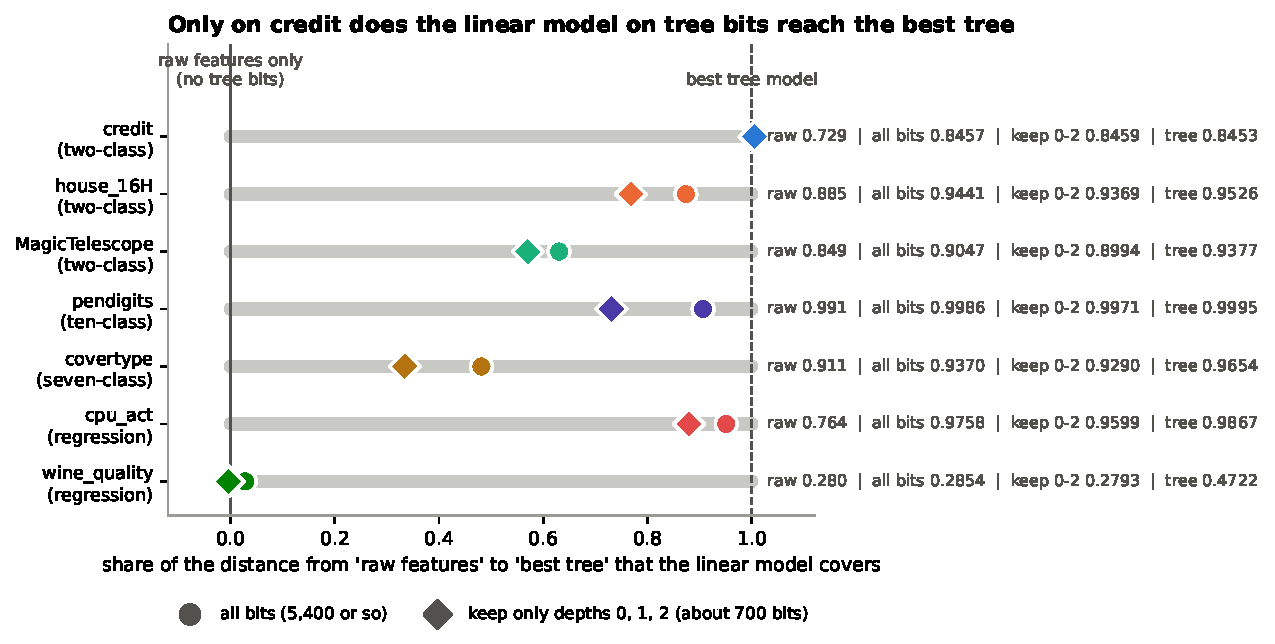
\includegraphics[width=0.95\textwidth]{fig1_position.pdf}
\caption{Where the linear model lands between ``raw features only'' and ``best
tree'' on each dataset. A circle at 1.0 means it reached the tree. Credit is
the only dataset where it does; on wine quality the bits add almost nothing a
linear model can use.}
\end{figure}

\begin{figure}[H]\centering
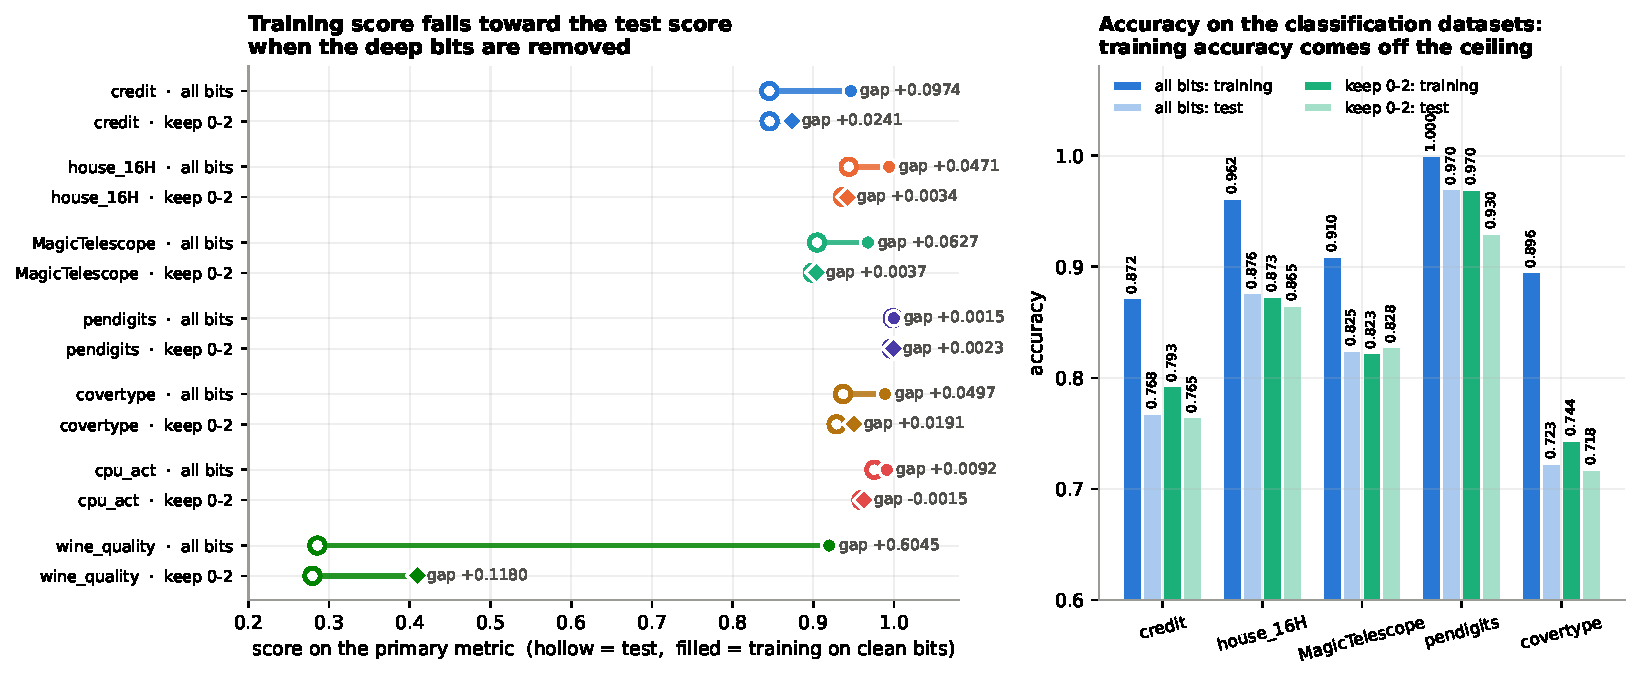
\includegraphics[width=\textwidth]{fig2_train_down.pdf}
\caption{Left: for every dataset, the training score (filled) and test score
(hollow) for the full encoding and for depths 0 to 2 only. The line between
them is the gap; it shortens on every dataset. Right: training and test
accuracy on the classification datasets. Training accuracy comes down from
its ceiling while test accuracy barely moves, except on the ten-class problem.}
\end{figure}

\begin{figure}[H]\centering
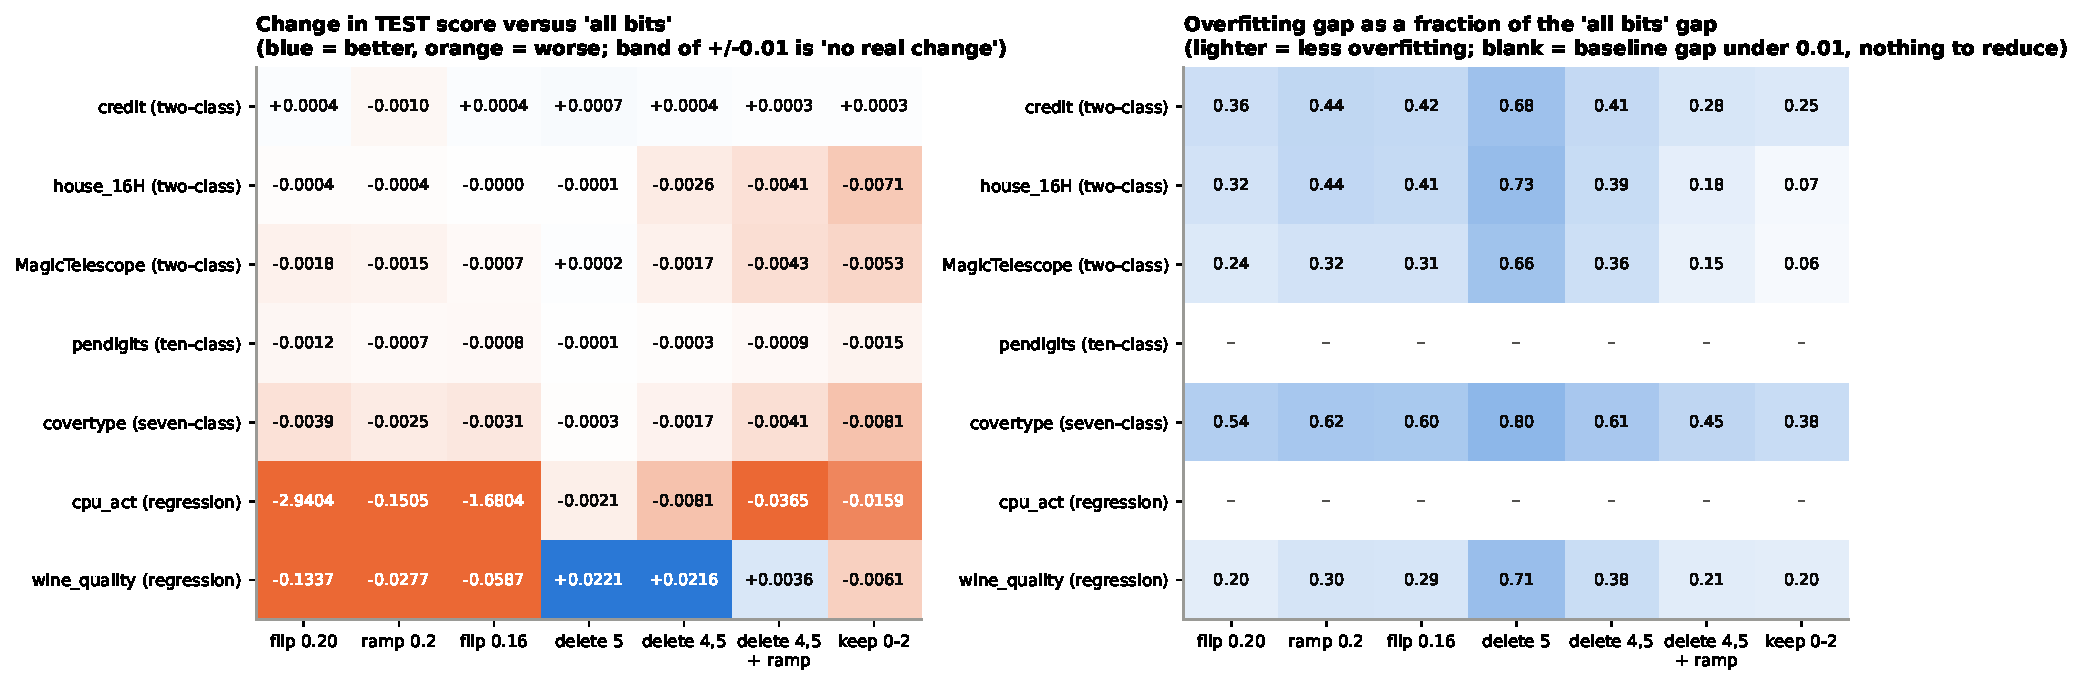
\includegraphics[width=\textwidth]{fig3_heatmaps.pdf}
\caption{Every arm on every dataset. Left: change in test score against the
baseline; values inside $\pm 0.01$ are not real differences. The two flat-noise
arms on cpu\_act are off the scale, at $-2.94$ and $-1.68$. Right: the gap as
a fraction of the baseline gap. Blank rows are the two datasets whose baseline
gap was under \num{0.01}, so there was nothing to reduce.}
\end{figure}

\begin{figure}[H]\centering
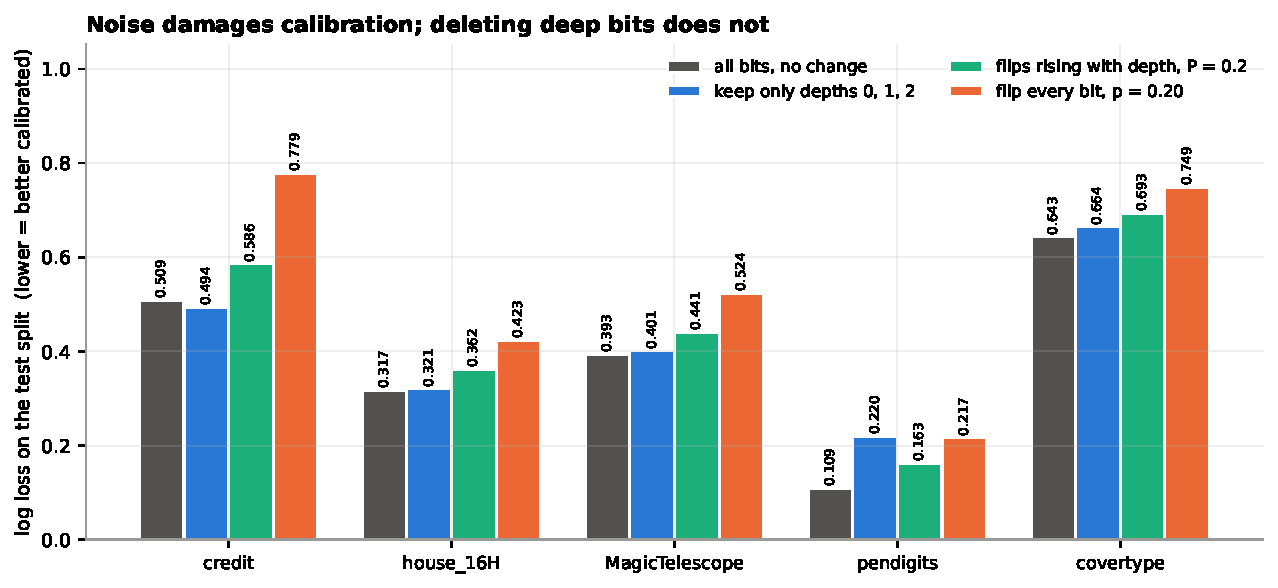
\includegraphics[width=0.85\textwidth]{fig4_calibration.pdf}
\caption{Log loss on the test split for the classification datasets. On the
two-class problems and on covertype, deleting depths leaves it roughly where it
was, while flipping bits raises it by 16 to 53 percent, meaning the model's
probabilities become less trustworthy even when its ranking does not change.
On the ten-class pendigits both deletion and noise double it.}
\end{figure}

\begin{figure}[H]\centering
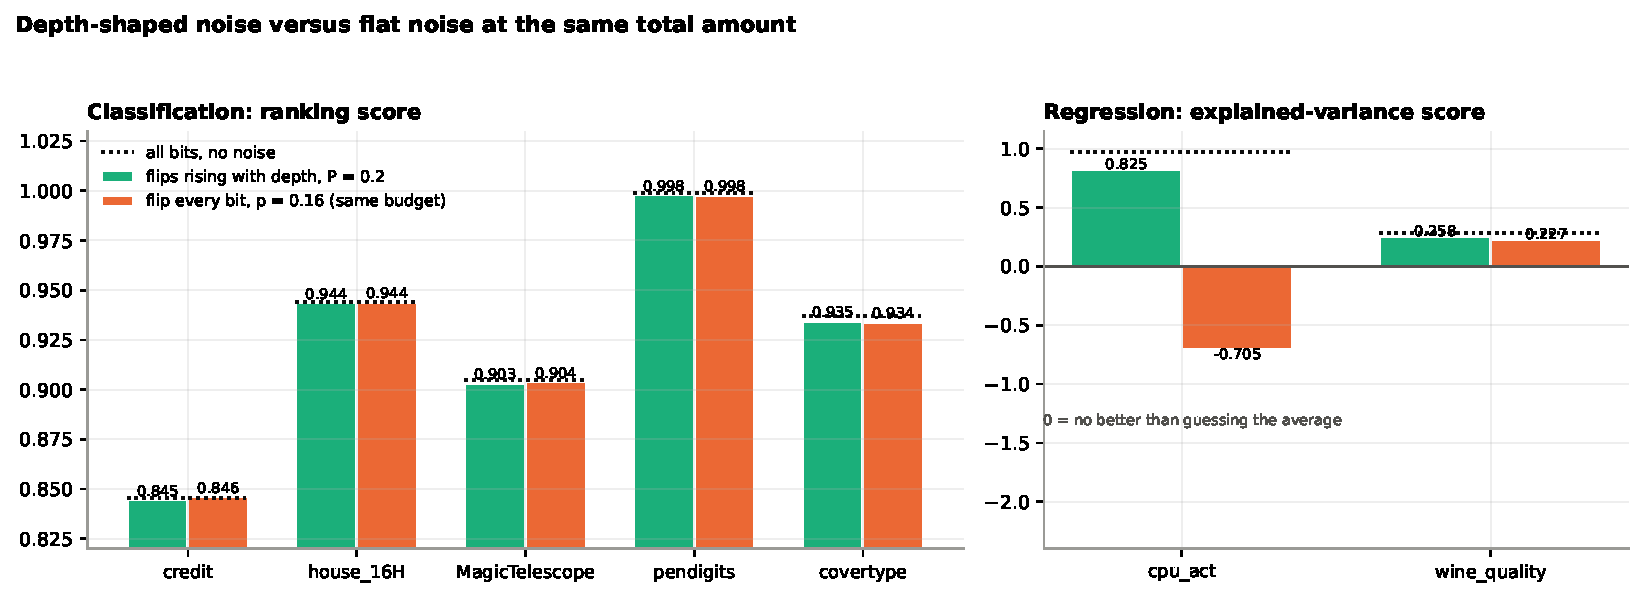
\includegraphics[width=\textwidth]{fig5_ramp_vs_flat.pdf}
\caption{The depth ramp beside the flat control that tells the same total
number of lies. On classification they tie. On regression, flat noise is
catastrophic, because it also flips the root bits that carry most of the
signal, and even the ramp costs a lot.}
\end{figure}

\clearpage
\subsection{Every arm on every dataset}

Each table lists all eight arms plus the raw-features floor and the best tree.
Training scores are on clean bits. The recommended arm from credit is in bold.

\begin{table}[H]\centering\footnotesize
\caption*{\textbf{credit} (two classes, the anchor dataset)}
\resizebox{\textwidth}{!}{\tabcredit}
\end{table}

\begin{table}[H]\centering\footnotesize
\caption*{\textbf{house\_16H} (two classes)}
\resizebox{\textwidth}{!}{\tabhouseSixteenH}
\end{table}

\begin{table}[H]\centering\footnotesize
\caption*{\textbf{MagicTelescope} (two classes)}
\resizebox{\textwidth}{!}{\tabMagicTelescope}
\end{table}

\begin{table}[H]\centering\footnotesize
\caption*{\textbf{pendigits} (ten classes)}
\resizebox{\textwidth}{!}{\tabpendigits}
\end{table}

\begin{table}[H]\centering\footnotesize
\caption*{\textbf{covertype} (seven classes)}
\resizebox{\textwidth}{!}{\tabcovertype}
\end{table}

\begin{table}[H]\centering\footnotesize
\caption*{\textbf{cpu\_act} (regression; typical error and average absolute error in percentage points of processor time)}
\resizebox{\textwidth}{!}{\tabcpuact}
\end{table}

\begin{table}[H]\centering\footnotesize
\caption*{\textbf{wine\_quality} (regression; errors in quality-score points)}
\resizebox{\textwidth}{!}{\tabwinequality}
\end{table}

\clearpage
\section{Observations}

\begin{enumerate}

\item \textbf{The observation holds on \nHolds{} of \nDatasets{} datasets, and
the two exceptions are exactly the two datasets that barely overfit to begin
with.} On pendigits the baseline gap is only \num{\pendigitsBaseGap} (training
ranking score \num{\pendigitsBaseTrain}, test \num{\pendigitsBaseTest}); there
is nothing to remove, and the shallow arm changes test by
\num{\pendigitsDTest}. On cpu\_act the baseline gap is \num{\cpuactBaseGap}
and the shallow arm removes it entirely (gap \num{\cpuactKeepGap}) but at a
test cost of \num{\cpuactDTest}, outside the tolerance. So the rule fails where
the premise fails: where there was no overfitting, feature regularisation had
no job to do.

\item \textbf{Wherever the model did overfit, deleting the deep layers cut the
gap by 62 to 94 percent.} Credit \num{\creditBaseGap} to \num{\creditKeepGap}
(\creditGapCut{} percent), house\_16H \num{\houseSixteenHBaseGap} to
\num{\houseSixteenHKeepGap} (\houseSixteenHGapCut{} percent), MagicTelescope
\num{\MagicTelescopeBaseGap} to \num{\MagicTelescopeKeepGap}
(\MagicTelescopeGapCut{} percent), covertype \num{\covertypeBaseGap} to
\num{\covertypeKeepGap} (\covertypeGapCut{} percent), wine\_quality
\num{\winequalityBaseGap} to \num{\winequalityKeepGap} (\winequalityGapCut{}
percent). The test score moved by at most \num{\covertypeDTest} on those five.

\item \textbf{The training score came down from its ceiling on every dataset.}
On the primary metric: credit \num{\creditBaseTrain} to
\num{\creditKeepTrain}, house\_16H \num{\houseSixteenHBaseTrain} to
\num{\houseSixteenHKeepTrain}, MagicTelescope \num{\MagicTelescopeBaseTrain}
to \num{\MagicTelescopeKeepTrain}, pendigits \num{\pendigitsBaseTrain} to
\num{\pendigitsKeepTrain}, covertype \num{\covertypeBaseTrain} to
\num{\covertypeKeepTrain}, cpu\_act \num{\cpuactBaseTrain} to
\num{\cpuactKeepTrain}, wine\_quality \num{\winequalityBaseTrain} to
\num{\winequalityKeepTrain}. Training \emph{accuracy}, the number asked about
directly: pendigits was literally \num{\pendigitsBaseTrainAcc} and came down
to \num{\pendigitsKeepTrainAcc}; house\_16H \num{\houseSixteenHBaseTrainAcc}
to \num{\houseSixteenHKeepTrainAcc}; covertype \num{\covertypeBaseTrainAcc}
to \num{\covertypeKeepTrainAcc}; credit \num{\creditBaseTrainAcc} to
\num{\creditKeepTrainAcc}; MagicTelescope \num{\MagicTelescopeBaseTrainAcc}
to \num{\MagicTelescopeKeepTrainAcc}. The model with 700 bits no longer
memorises the training set.

\item \textbf{Credit is the only dataset where the linear model matches the
best tree.} Measured as the share of the distance from ``raw features only'' to
``best tree'' that the full encoding covers: credit \creditClosed{} percent
(\num{\creditBaseTest} against a tree of \num{\creditTree}), cpu\_act
\cpuactClosed{} percent, pendigits \pendigitsClosed{} percent, house\_16H
\houseSixteenHClosed{} percent, MagicTelescope \MagicTelescopeClosed{}
percent, covertype \covertypeClosed{} percent, wine\_quality
\winequalityClosed{} percent. The bits carry a large part of what the trees
know, but on six of seven datasets a linear read-out of them does not recover
all of it. The earlier ``matches the tree'' headline was a property of credit.

\item \textbf{Wine quality is the clearest case of memorisation without
learning.} With all bits the training explained-variance score is
\num{\winequalityBaseTrain} and the test score \num{\winequalityBaseTest}, a
gap of \num{\winequalityBaseGap}. The raw features alone reach
\num{\winequalityRaw}, so the \num{\winequalityBits} bits added almost nothing
a linear model could use, while giving it enough capacity to fit the training
set nearly perfectly. The best tree reaches \num{\winequalityTree}; whatever it
knows about wine is not linear in these bits. Here deletion even
\emph{improves} test: deleting depth 5 gives \num{\winequalityDropFiveTest},
the best arm on this dataset.

\item \textbf{Deleting regularises cleanly; flipping damages calibration.}
Log loss on the test split, the penalty for confident wrong answers, tells the
two apart. Baseline, shallow, and flip-every-bit-at-0.20: credit
\num{\creditBaseLL}, \num{\creditKeepLL}, \num{\creditUnifLL}; house\_16H
\num{\houseSixteenHBaseLL}, \num{\houseSixteenHKeepLL},
\num{\houseSixteenHUnifLL}; MagicTelescope \num{\MagicTelescopeBaseLL},
\num{\MagicTelescopeKeepLL}, \num{\MagicTelescopeUnifLL}; covertype
\num{\covertypeBaseLL}, \num{\covertypeKeepLL}, \num{\covertypeUnifLL}.
On these four, deletion leaves the probabilities about as trustworthy as
before while flipping makes them 16 to 53 percent worse, even though the
ranking score is unchanged. Pendigits is the exception: baseline
\num{\pendigitsBaseLL}, shallow \num{\pendigitsKeepLL}, flipped
\num{\pendigitsUnifLL}; there both deletion and noise double the log loss,
consistent with the many-class point below. The reason is a mismatch: the model is fitted on bits that are on
more often than the clean bits it is scored on, so its scores shift. Ranking
ignores a shift; log loss does not.

\item \textbf{The same mismatch is catastrophic for regression.} Flat noise at
$p = 0.16$ drives cpu\_act from \num{\cpuactBaseTest} to
\num{\cpuactCtrlTest}, worse than guessing the average, and at $p = 0.20$ to
\num{\cpuactUnifTest}. On wine\_quality flat noise at 0.16 gives
\num{\winequalityCtrlTest} against a baseline of \num{\winequalityBaseTest}.
A shifted score that ranking tolerates is a wrong number that a
number-prediction score punishes in full.

\item \textbf{The depth shape of the noise does not matter for classification
and matters enormously for regression.} Ramp against its equal-budget flat
control on the five classification datasets: credit \num{\creditRampTest}
against \num{\creditCtrlTest}, house\_16H \num{\houseSixteenHRampTest} against
\num{\houseSixteenHCtrlTest}, MagicTelescope \num{\MagicTelescopeRampTest}
against \num{\MagicTelescopeCtrlTest}, pendigits \num{\pendigitsRampTest}
against \num{\pendigitsCtrlTest}, covertype \num{\covertypeRampTest} against
\num{\covertypeCtrlTest}, every pair within \num{0.0015}. On regression the
ramp is far better, cpu\_act \num{\cpuactRampTest} against
\num{\cpuactCtrlTest} and wine\_quality \num{\winequalityRampTest} against
\num{\winequalityCtrlTest}, because it never flips the root bits that carry
most of a regression forest's signal. But even the ramp costs cpu\_act
\num{0.15} of explained variance. Noise, of any shape, is the wrong tool for
regression; deletion is the right one.

\item \textbf{Many-class problems keep more of their signal in the deep bits.}
On pendigits the shallow arm loses only \num{0.0015} of ranking score but
\num{0.040} of accuracy (\num{\pendigitsBaseTestAcc} to
\num{\pendigitsKeepTestAcc}), because telling ten digits apart needs the fine
splits that deep bits provide. Covertype shows the same in milder form
(\num{\covertypeBaseTestAcc} to \num{\covertypeKeepTestAcc}). Ranking score
alone would have hidden this; tracking every metric on every split exposed it.

\item \textbf{How much to delete is a dial, and the dial reads the same on
every dataset.} Deleting only depth 5 never costs more than \num{0.0021} of
test score on any dataset and cuts the gap by 20 to 34 percent. Deleting
depths 4 and 5 costs at most \num{0.0081} and cuts the gap by 39 to 64
percent. Keeping only depths 0 to 2 costs at most \num{0.0159} and cuts it by
62 to 94 percent. More deletion buys more regularisation at a slowly rising
price, with the price highest on regression and many-class problems.

\item \textbf{Every number here is from one random split and one seed.} The
noise arms were shown earlier to vary by only \num{0.0002} between fresh noise
draws, but the split itself is a larger source of variation, roughly
\num{0.01} on a test set of two thousand rows. Differences smaller than that
between arms should be read as ties.

\end{enumerate}

\section{Key findings}

\begin{enumerate}

\item \textbf{Feature regularisation works as a regulariser across every kind
of problem tested.} On all five datasets where the full encoding overfit,
deleting the deep tree layers cut the train-minus-validation gap by 62 to 94
percent and brought the training score off its ceiling, at a test cost of at
most \num{0.008} for deleting two layers and \num{0.016} for keeping only
three. The credit observation was not a fluke of credit.

\item \textbf{The ``linear model matches the tree'' result was specific to
credit.} On the other six datasets the linear model covers between 48 and 95
percent of the way from raw features to the best tree, and on wine quality
almost none. The tree models remain ahead on six of seven datasets. The
encoding carries most of what the trees know; a linear read-out does not
recover all of it. This qualifies the earlier report and should be stated
plainly in anything written up.

\item \textbf{Delete, do not flip.} Deletion has far smaller side effects
than noise. On two-class problems it leaves calibration and test scores intact;
on regression and many-class problems it costs a little, never more than
\num{0.016} of test score. Bit-flip noise raises log loss by 16 to 98 percent
on classification, is destructive on regression, and never beats deletion on
the test score. The recommended default is to delete depths 4 and 5, which
shrinks the encoding three to four times, cuts overfitting by 39 to 64 percent,
and costs at most \num{0.008} anywhere. On
two-class problems, keeping only depths 0 to 2 is free and cuts overfitting
by 75 to 94 percent.

\item \textbf{Depth-shaped noise is not worth pursuing.} Against an
equal-budget flat control it ties on every classification dataset. It wins on
regression only because flat noise is catastrophic there, and even then it
loses badly to simple deletion. The intuition behind it, that deep splits are
the unreliable ones, is correct, and the way to act on it is to delete them.

\item \textbf{Track more than one score.} The ranking score alone would have
said the shallow encoding is free on pendigits; accuracy shows it costs four
points. The ranking score alone would have said noise is harmless on
classification; log loss shows it damages the probabilities. The request to
track all metrics on all splits changed the conclusions, not just the tables.

\item \textbf{What this establishes, and what comes next.} With the feature
side now characterised across task types, the next step named in the earlier
discussion is to put richer heads on the shallow encoding and compare them
against this logistic one under the identical protocol. The tree models' lead
on six of seven datasets says a nonlinear head has real room to gain; the
credit result says it should be judged against a linear baseline that is
already strong.

\end{enumerate}

\vfill
\begin{flushleft}\footnotesize
\textbf{Reproduction.} One command runs everything and writes every table,
figure and per-run log:\\
\texttt{python run\_feature\_reg\_suite.py -{}-root results/featreg\_suite -{}-bundle}\\[2pt]
Repository: \texttt{github.com/sushanedulloo/TKCE}. Driver notebook:
\texttt{colab\_feature\_reg\_suite.ipynb}. All numbers in this document,
including those in the text, are generated from the run's own result files;
none was typed by hand.
\end{flushleft}

\end{document}
